\documentclass[10pt,twocolumn,letterpaper]{article}

\usepackage{../common/cvpr}
\usepackage{times}
\usepackage{epsfig}
\usepackage{graphicx}
\usepackage{amsmath}
\usepackage{amssymb}
\usepackage[normalem]{ulem}
\useunder{\uline}{\ul}{}

% Include other packages here, before hyperref.

% If you comment hyperref and then uncomment it, you should delete
% egpaper.aux before re-running latex.  (Or just hit 'q' on the first latex
% run, let it finish, and you should be clear).
\usepackage[pagebackref=true,breaklinks=true,letterpaper=true,colorlinks,bookmarks=false]{hyperref}

\cvprfinalcopy % *** Uncomment this line for the final submission

% Pages are numbered in submission mode, and unnumbered in camera-ready
\ifcvprfinal\pagestyle{empty}\fi
\begin{document}

%%%%%%%%% TITLE
\title{Mastering Terra Mystica: Super-human Strategy in AI}

%\author{
%Luis Perez\\
%Stanford University\\
%450 Serra Mall\\
%{\tt\small luisperez@cs.stanford.edu}
%}

\maketitle
\thispagestyle{empty}

%%%%%%%%% ABSTRACT
\begin{abstract}
In this paper, we explore and compare multiple algorithms for solving the complex strategy game of Terra Mystica, thereafter abbreviated as TM. Previous work in the area of super-human game-play using AI has proven effective, with recent break-throughs for generic algorithms in games such as Go, Chess, and Shogi \cite{AlphaZero}. We directly apply these breakthroughs to a novel state-representation of TM by combining multiple techniques to create an AI capable of rivaling human players. Specifically, we present initial results of applying AlphaZero to this state-representation, and analyze the strategies developed, their strengths and weakness. We call this modified algorithm with our novel state-representaiton AlphaTM. In the end, we discuss the success and short-comings of this method by comparing against multiple baselines and typical human scores.
\end{abstract}

%%%%%%%%% BODY TEXT
\section{Task Definition}
\label{section:task_definition}
Our proposal involves developing the infrastructure, framework, and models required to achieve super-human level game-play in the game of Terra Mystica (TM).  The game of TM involves very-little luck, and is entirely based on strategy (similar to Chess, Go, and other games which have recently broken to novel Reinforcement Learning such Deep Q-Learning and Monte-Carlo Tree Search as a form of Policy Improvement \cite{AlphaGo} \cite{AlphaGoZero}). In fact, any random component to the game comes only from the initial configuration of the map and the initial reward structure, which is selected at random during typical game-play.

TM is a game played between 2-5 players. For our research, we focus mostly on the adversarial 2-player version of the game. We do this mostly for computational efficiency, though for each algorithm we present, we discuss briefly strategies for generalizing them to multiple players.

TM is a fully-deterministic game whose complexity arises from the large branching factor and a large number of possible actions $A_t$ from a given state, $S_t$. There is further complexity caused by the way in which actions can interact, discussed further in Section \ref{subsection:input/output_of_system}.

\subsection{Input/Output Of System}
\label{subsection:input/output_of_system}
In order to understand the inputs and outputs of our system, the game of TM must be fully understood. We lay out the important aspects of a given state below, according to the standard rules \cite{TMRules}..

The game of TM consists of a terrain board that's split into $9 \times 13$ terrain tiles. The board is fixed, but each terrain tile can be terra-formed (changed) into any of the 7 distinct terrains (plus water, which cannot be modified). Players can only expand onto terrain which belongs to them. Furthermore, TM also has a mini-game which consists of a Cult-Board (see Figure \ref{fig:TM_Cult_Track}) where individual players can choose to move up in each of the cult-tracks throughout game-play. 

The initial state of the game consists of players selecting initial starting positions for their original dwellings. 

At each timestep, the player has a certain amount of resources, consisting of Workers, Priests, Power, and Coin. The player also has an associated number of VPs.

Throughout the game, the goal of each player is to accumulate as many VPs as possible. The player with the highest number of VPs at the end of the game is the winner.

From the definition above, the main emphasis of our system is the task of taking a singe state representation $S_t$ at a particular time-step, and outputting an action to take to continue gameplay for the current player. As such, the input of our system consists of the following information, fully representative of the state of the game:

\begin{enumerate}
    \item Current terrain configuration. See Figure \ref{fig:TM_Board} for a reference. The terrain configuration consists of multiple pieces of information. For each terrain tile, we will receive as input:
    \begin{enumerate}
        \item The current color of the tile. This gives us information not only about which player currently controls the terrain, but also which terrains can be expanded into.
        \item The current level of development for the terrain. For the state of development, we note that each terrain tile can be one of (1) UNDEVELOPED, (2) DWELLING, (3) TRADING\_POST, (4) SANCTUARY, or (5) STRONGHOLD.
        \item The current end-of-round bonus as well as future end-of-round bonus tiles.
        \item Which special actions are currently available for use.
    \end{enumerate}
    \item For each player, we also receive the following information.
    \begin{enumerate}
        \item Current level of shipping ability, Current level of spade ability, the current number of VPs that the player has.
        \item The current number of towns the player has (as well as which town is owned), The current number of worker available to the player, the current number of coins available to the player, the current number of LV1, LV2, and LV3 power tokens.
        \item The current number of priests available to the player.
        \item Which bonus tiles are currently owned by the player.
        \item The amount of income the player currently produces. This is simply the power, coins, priests, and worker income for the player.
    \end{enumerate}
\end{enumerate}

The above is an incomplete enumeration of the input to our algorithm, and has not yet been fully formalized. However, in general, the input to the algorithm is a complete definition of the game state at a particular turn. Note that Terra Mystica \textit{does not} have any dependencies in previous moves, and is completely Markovian. As such, modeling the game as an MDP is fully realizable, and is simply a question of incorporating all the features of the state.

\subsection{Output and Evaluation Metrics}
For a given state, the output of our algorithm will consist of an action which the player can take to continue to the next state of the game. Actions in TM are quite varied, and we do not fully enumerate them here. In general, however, there are eight possible actions:
\begin{enumerate}
    \item Convert and build.
    \item Advance on the shipping ability.
    \item Advance on the spade ability.
    \item Upgrade a building.
    \item Sacrifice a priest and move up on the cult track.
    \item Claim a special action from the board.
    \item Some other special ability (varies by class)
    \item Pass and end the current turn.
\end{enumerate}

We will evaluate our agents using the standard simulator. The main metric for evaluation will be the maximum score achieved by our agent in self-play when winning, as well as the maximum score achieved against a set of human competitors.

\section{Infrastructure}
An open-source simulator for the game of TM already exists and is written in TM \cite{infra}. We've currently converted this open-source simulator into Python and can run locally, simulating gameplay. For our baselines, we've taken the built-in AI agents as baselines (which tend to perform relatively poorly). For our oracles, we've instead taken the approach of analyzing a large database of game data available online.

\subsection{Overview of Model and Approaches}
Developing an AI agent that can play well will be extremely challenging. Even current heuristic-based agents have difficulty scoring positions. The state-action space for TM is extremely large. Games typically have trees that are $>50$ moves deep (per player) and which have a branching factor of $>10$. 

We can approach this game as a typical minmax search-problem. Simple approaches would simply be depth-limited alpha-beta pruning similar to what we used in PacMan. These approaches can be tweaked for efficiency, and are essentially what the current AIs use.

Further improvement can be made to these approaches by attempting to improve on the $Eval$ functions.

However, the main contribution of this paper will be to apply more novel approaches to a custom state-space representation of the game. In fact, we will be attempting to apply Q-Learning -- specifically DQNs (as per \cite{AlphaGo}, \cite{AlphaGoZero}, and \cite{AlphaZero}). 

\section{Baselines}
For the base-lines, we have quite a few options. Using the simulator that's been converted into Python, we already have multiple AI agents that have been developed and can be played against. We can use these as the lowest bound for the baselines, since even the strongest-AI agents so far struggle to complete against average TM players. We summarize the results for these agents in Table 1.

\section{Oracle}
For an Oracle, we have two options. Even the current state-of the art AI in TM does not come close to beating average TM players. However, there is a large collection of online games that have been played by humans \cite{TMStats}. From these statistics, we can derive the following-upper bounds.

\subsection{Competitive Player Oracle}
Our oracle will therefore consists of the scores achieved by expert players. We've summarized this data in Table \ref{table:average_2p_score}, broken down by faction. We look only at the two-player scenario, as this is the one on which our algorithm focuses.

\section{Deep Q-Learning Methods for Terra Mystica}
In this section, we describe the main methods we use for training our agent. In particular, we place heavy emphasis on the methods described by AlphaGo\cite{AlphaGo}, AlphaGoZero, \cite{AlphaGoZero}, and AlphaZero \cite{AlphaZero} with pertinent modifications made for our specific problem domain.


\subsection{AlphaTMZero}
Our main method will be a modication of the AlphaGo Zero \cite{AlphaGoZero} algorithm which was described in detail. We chose this algorithm over the methods described for Alpha Go \cite{AlphaGo} for two main reasons -- the AlphaGo Zero is a zero-knowledge reinforcement learning algorithm. This means that it requires to expert human play data and rather both generates (simulates gameplay) as well as 

We describe an adaptation of the AlphaGoZero algorithm which we're implementing. Given how generic the algorithm is, we'll be mostly implementing a simple modifications to it, consisting almost exclusively of how we modify the input and the output.



\section{Preliminary Results}
We've run only a few experiments, many of which demonstrate severe limitations of our model and possible our infrastructure. We're focusing exclusively.

TODO(LEARNING RATE AND OTHER CRAP WITH THE MODEL IN SEVERELY RESTRICTED MODE!!!! UGH)

\section{Appendices}
% This section is optional. Include additional derivations of proofs which weren’t core to the understanding of your proposed algorithm. Usually you put equations here when you don't want to disrupt the flow of the main paper.
%Optional. More details to be added later.

\begin{table}[h!]
\begin{tabular}{|l|l|l|}
\hline
\multicolumn{3}{|c|}{{\ul \textbf{Average Human Score (2p)}}}      \\ \hline
\textbf{Faction} & \textbf{Average Score} & \textbf{Sampled Games} \\ \hline
Darkling         & 137.10                 & 2496                   \\ \hline
Swarmling        & 132.93                 & 2302                   \\ \hline
Chaos Magician   & 130.06                 & 2621                   \\ \hline
Halfing          & 133.32                 & 2227                   \\ \hline
Auren            & 122.74                 & 964                    \\ \hline
Cultists         & 123.25                 & 702                    \\ \hline
Alchemist        & 127.48                 & 1443                   \\ \hline
Witches          & 127.44                 & 2124                   \\ \hline
Engineers        & 127.72                 & 1543                   \\ \hline
Mermaids         & 125.11                 & 1700                   \\ \hline
Giants           & 122.16                 & 975                    \\ \hline
Nomads           & 121.15                 & 2291                   \\ \hline
Dwarves          & 123.58                 & 1054                   \\ \hline
Fakirs           & 119.16                 & 629                    \\ \hline
\end{tabular}
\caption{Average human scores by faction for a two-player TM games online.}
\label{table:average_2p_score}
\end{table}

\begin{table}[h!]
\begin{tabular}{|l|l|l|}
\hline
\multicolumn{3}{|c|}{{\ul \textbf{Simulated Self-Play Average Scores}}}      \\ \hline
\textbf{Faction} & \textbf{Average Score} & \textbf{Sampled Games} \\ \hline
Darkling         & 90.10                 & 1000                   \\ \hline
Swarmling        & 93.12                 & 1000                   \\ \hline
Chaos Magician   & 61.44                 & 1000                   \\ \hline
Halfing          & 92.21                 & 1000                   \\ \hline
Auren            & 91.74                 & 1000                    \\ \hline
Cultists         & 93.11                 & 1000                    \\ \hline
Alchemist        & 72.12                 & 1000                   \\ \hline
Witches          & 79.89                 & 1000                   \\ \hline
Engineers        & 77.12                 & 1000                   \\ \hline
Mermaids         & 85.11                 & 1000                   \\ \hline
Giants           & 85.11                 & 1000                    \\ \hline
Nomads           & 99.9                 & 1000                   \\ \hline
Dwarves          & 90.11                 & 1000                   \\ \hline
Fakirs           & 82.19                 & 1000                    \\ \hline
\end{tabular}
\caption{Self-play easy AI agent: AI\_Level5 from \cite{TMStatsAI}}
\label{table:average_2p_score}
\end{table}

\begin{figure}[h!]
    \centering
    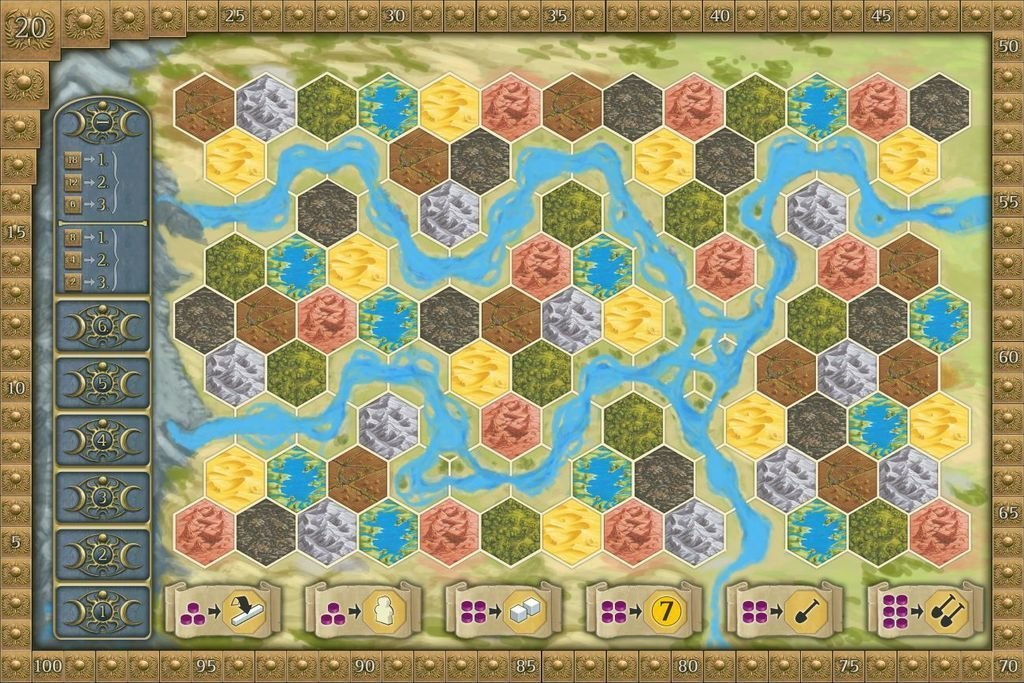
\includegraphics[scale=0.2]{../figures/tm_board}
    \caption{The Terra Mystyca Game Board and Its Representation}
    \label{fig:TM_Board}
\end{figure}

\begin{figure}[h!]
    \centering
    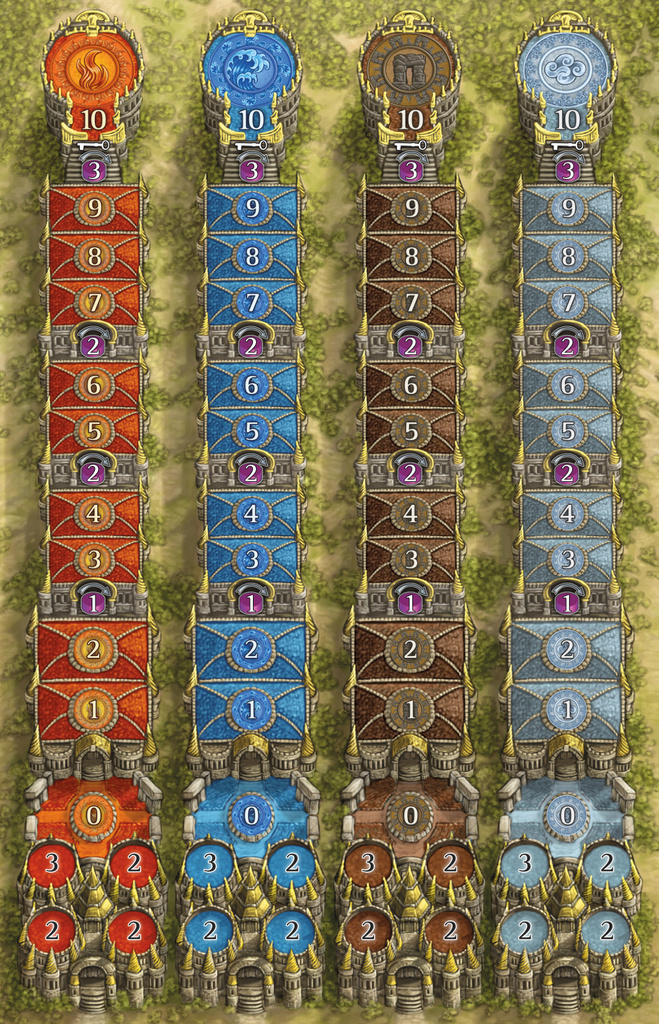
\includegraphics[scale=0.6]{../figures/terra-mystica-cult}
    \caption{The Terra Mystyca Cult Track}
    \label{fig:TM_Cult_Track}
\end{figure}

{\small
\bibliographystyle{../common/ieee}
\bibliography{../common/egbib}
}

\end{document}
